% TeX root = ../main.tex
\chapter{Fourier Series}

  Throughout this chapter we will be concerned with periodic functions. We will discuss the Fourier series of functions and their convergence. Before we begin we will formally define periodic functions in $\R$. 
  \begin{definition}[Periodic function]
    \label{def:periodic_function}
    A function $f:\R \to \R$ is called periodic with period $p$ (or $p$-periodic) if $f(x+p) = f(x)$ for all $x \in \R$
  \end{definition}

  From the above definition it is evident that a periodic function in $\R$ is uniquely determined by the its images in a closed open interval of length $p$, where $p$ is the period of the function. Moreover if $g: \R \to \R$ is a $p$-periodic function, $f(x) := g(\frac{x}{p})$ is a $1$-periodic function. Thereofore we'll focus our attention to $1$-periodic function. Now we'll identifiy $1$-periodic functions in $\R$ with functions in the interval $[0,1)$. By this identification we will be able to use many results from Lebesgue measure theory which are restricted to finite measure spaces.

  \section{Structure and Topology of $\T$}
 % \label{def:definition_of_T}
  Let us define an relation $\sim$ on $\R$ where $$x \sim y \iff x-y \in \Z$$
  It is easy to verify that this is an equivalence relation on $\R$ and the equivalence classes of this relation is denoted by $\T$ or $\frac{\R}{\Z}$. Note that if $r \in \R$, then the equivalence class of $r$, denoted by $[r]$ is $$[r] = r + \Z = \left\{r + n \ \vert \ n \in \Z \right\} = \{r\} + \Z$$
 where $\{r\}$ is the fractional part of $r$. 

  Moreover $f: \R \to \T$ defined as $f(r) = [r]$ is a surjective map onto $\T$ and therefore defines the quotient topology on $\T$. 


% By our identification of $T$ with $[0, 1)$ this translates to the quotient topology on $[0, 1)$ given by the map $\tilde{f} : \R \to [0, 1)$ as $\tilde{f}(r) = \{r\}$.
% Now $\T$ can be identified with $[0, 1)$ where $[r] \in \T$ is identified with $\{r\} \in [0, 1)$. Therefore by abuse of notation we'll use $\T = [0, 1)$ instead of $\frac{\R}{\Z}$

  \begin{proposition}[Periodisation of functions in $\T$]
   Let $f: \R \to \R$ be defined as $f(x) = [x]$ and $h: \T \to \R$. Then $h \circ f: \R \to \R$ is a periodic function of period $1$.
  \end{proposition}

By the above theorem we consider functions in $\T$ as $1$-periodic functions in $\R$. Also, having endowed $\T$ with a topology and measure, we are now at a position to discuss continuity of functions in $\T$.

\begin{proposition}[Continuous functions in $\T$]
  \label{prop:continuous_functions_on_T}
  Let $g : \T \to \R$ be a function. Then $g$ is continuous on $\T$ if and only if the function $h: \R \to \R$ defined as $h(x) = g([x])$ is a continuous function of period $1$.
\end{proposition}
\begin{proof}
  ($\implies$) Assume $g$ is a continuous function in $\T$. Then by the definition, if $U \subset \R$ is an open set then $g^{-1}(A)$ is an open set in $\T$. Since the topology on $\T$ is defined by the quotient map $f: \R \to \T$, where $f(x) = [x]$, we get that $f^{-1}g^{-1}(A)$ is open in $\R$. Since $h = g \circ f$ by definition, it follows that $h$ is continuous. Also since $f(x + 1) = f(x)$ for all $x \in \R$, it follows that $h$ is of period $1$.

  ($\impliedby$) Assume that $h$ is a continuous function on $\R$. Then $h^{-1}(A)$ is an open set in $\R$ for any open set $A \in \R$. Since $h = g \circ f$ we get $f^{-1}g^{-1}(A)$ is open in $\R$. Again since $f$ is a quotient map to $\T$, we get that $g^{-1}(A)$ is open in $\T$. Therefore $g$ is a continuous function on $\T$.
\end{proof}

Now by abuse of notation we'll identify $\T$ with $[0, 1)$ by the function $f:[x] \to \{ x \}$. By this identification we can define Lebesgue measure on $\T$. If $A$ is an open subset of $\T$ then Lebesgue measure of $A$ is defined as, $\mu(A) = \lambda(f(A))$ where the $\lambda$ is the Lebesgue measure on $\R$. Then we see that $\T$ is a finite Lebesgue measure space.

Recall the definition of $L^p$ funtions for a Lebesgue measure space.
  \begin{definition}[$L^p$ function]
    \label{def:Lp_function}
    A real valued function $f$ defined on a Lebesgue measure space $S$ is called an $L^p$ function on $S$ or a $p$-integrable function on $S$ if 
    \begin{displaymath}
       \left( \int_{S} |f(x)|^p d\mu \right)^{1/p} < \infty
    \end{displaymath}
    For such a function the integral above is called the $p$-norm of the function $f$ and often denoted by $\|f\|_{L^p(S)}$ or $\|f\|_p$ if the space is known.
  \end{definition}

Let us now prove an important result about periodic functions.
  \begin{lemma}
    \label{lem:integral_of_periodic_function}
    If $f:\R \to \R$ is of period $1$ and $\int_{0}^{1} f(x) dx$ exists, then for any real number $a$, 
    \begin{displaymath}
      \int_{a}^{a+1}f(x) dx = \int_{0}^{1} f(x) dx
    \end{displaymath} 
  \end{lemma}
  \begin{proof}
    Let $a = n +b$, where $0\le b <1$ and $n$ is an integer. Then since $f$ has period 1,
      $\int_{a}^{a+1}f(x) dx = \int_{n+b}^{n+b+1}f(x)dx = \int_{b}^{b+1}f(x+n)dx = \int_{b}^{b+1}f(x)dx $
    and, 
    \begin{align*}
      \int_{b}^{b+1}f(x)dx &= \int_{b}^{1}f(x)dx + \int_{1}^{b+1}f(x)dx \\
                      &= \int_{b}^{1}f(x)dx + \int_{0}^{b}f(x+1)dx \\
                      &= \int_{b}^{1}f(x)dx + \int_{0}^{b}f(x)dx \\
                      &= \int_{0}^{1}f(x)dx
    \end{align*}
    Hence the result.
  \end{proof}


  \section{Fourier Coefficients}
  Now we'll define fourier coefficients of a periodic function $f \in L^1(\T)$
  \begin{definition}[Fourier coefficient]
    \label{def:fourier_coefficient}
    Let $f \in L^1(\T)$, i.e $\int_{\T} f < \infty$. Then for each integer $n$ we define the $n^{th}$ fourier coefficient, $\hatf(n)$ as 
    \begin{displaymath}
      \hatf(n) = \int_0^1 f(x)e^{-2\pi inx} dx \end{displaymath}
  \end{definition}
  $\hatf(n)$ is finite and well defined for each $n$ since $f \in L^1(\T)$, since
  \begin{align*}
    |\hatf(n)| &\le \int_0^1 |f(x)e^{-2\pi inx}| dx \\
               &\le \int_0^1 |f(x)||e^{-2\pi inx}| dx \\
               &= \int_0^1|f(x)| dx < \infty
  \end{align*}
  
  Once we have the fourier coefficients of a function at hand we can combine them together to make a series called the fourier series. We'll be investigating the conditions at which this series converges to our initial function $f$.

  Also note that the map which takes $f$ to $\hatf$ is linear since if $f, g \in L^1(\T)$, then 
  \begin{align*}
    \widehat{f+g}(n) &= \int_0^1 (f+g)(x) e^{-2 \pi inx} \ dx \\
              &= \int_0^1f(x)e^{-2\pi inx} \ dx + \int_0^1 g(x)e^{-2\pi inx} \ dx \\
              &= \hatf(n) + \hatg(n)
  \end{align*}
  and for $\lambda \in \R$
  \begin{align*}
  \widehat{\lambda f}(n) \ dx &= \int_0^1 \lambda f(x) e^{-2\pi inx} \ dx \\
              &= \lambda \int_0^1 f(x) e^{-2 \pi inx} \ dx \\
              &= \lambda\hatf(n)
  \end{align*}

  \begin{definition}[Fourier series]
    \label{def:fourier_series}
    Given a function $f \in L^1(\T)$, the fourier series of the function $f$ is defined as 
    \begin{displaymath}
      \sum_{n\in \Z} \hatf(n)e^{2\pi inx}
    \end{displaymath}
    where $\hatf(n)$ is the $n^{th}$ fourier coefficient as \autoref{def:fourier_coefficient} 
  \end{definition}

  \begin{proposition}[Properties of Fourier coefficients]
    \label{prop:properties_of_fourier_coefficients}
    Suppose that $f\in L^1(\T)$.
    \begin{enumerate}[label=(\alph*)]
      \item If $a$ is a real number and $g(x) = f(x+a)$ for all $x$, then $\hatg(n) = \hatf(n)e^{2\pi ina}$ for all $n \in \Z$.
      \item If $b$ is an integer and $h(x) = f(x)e^{2\pi i bx}$ for all $x$, then $\hath(n) = \hatf(n-b)$ for all $n\in \Z$.
      \item If $j(x) = f(-x)$ for all $x$, then $\hatj(n) = \hatf(-n)$
    \end{enumerate}
  \end{proposition}
  \begin{proof}
     Given $f(x) \in L^1(\T)$ and $n^{th}$ Fourier coefficient of $f$,  
    \[\hatf(n) = \int_{0}^{1}f(x)e^{-2 \pi inx}.\]
    \begin{enumerate}
      \item[(a)] Then, the $n^{th}$ Fourier coefficient of $g(x) = f(x+a)$ is
        \begin{align*}
          \hatg(n) &= \int_{0}^{1}g(x)e^{-2\pi inx} dx \\
                &= \int_{0}^{1}f(x+a)e^{-2\pi inx} dx \\
                &= \int_{0}^{1}f(x)e^{-2\pi in(x-a)} dx \\
                &= e^{2\pi ina} \int_0^1 f(x)e^{-2\pi inx} dx \\
                &= e^{2\pi ina} \hatf(n)
        \end{align*}

      \item[(b)] If $h(x) = f(x)e^{2\pi ibx}$, then
        \begin{displaymath}
          \hath(n) = \int_0^1 f(x)e^{-2 \pi i (n-b)x} dx = \hatf(n-b)
        \end{displaymath}
      \item[(c)] $j(x) = f(-x)$, then
        \begin{align*}
          \hatj(n)  &= \int_0^1 f(-x)e^{-2\pi inx} dx \\
                    &= -\int_0^{-1} f(y) e^{2\pi iny}dy & \text{by } y=-x\\
                    &= \int_{-1}^0 f(y)e^{2\pi iny}dy \\
                    &= \int_0^1 f(y)e^{2\pi iny}dy & \text{by \autoref{lem:integral_of_periodic_function}}\\
                    &= \hatf(-n)
        \end{align*}
    \end{enumerate}
  \end{proof}


  \section{Convolution}
  Now we'll define another important operation with function called the convolution of two functions.
  \begin{definition}
    \label{def:convolution_of_functions_in_L^1(T)}
    Let $f, g \in L^1(\T)$, then the convolution of $f$ and $g$ is defined as 
    \begin{displaymath}
      f*g(x) = \int_0^1 f(x-y)g(y)dy
    \end{displaymath}
  \end{definition}

  % Convolution can be thought of as taking the moving average of a function with another function. Refer \autoref{fig:convolution}.
  % \begin{figure}
  %   \centering
  %   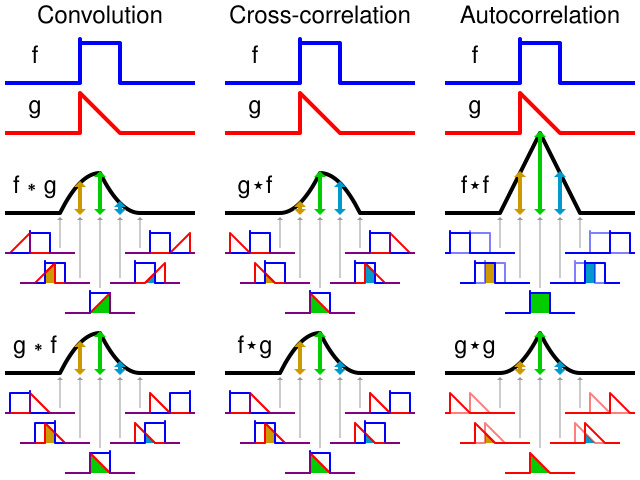
\includegraphics[width=0.6\textwidth]{convolution}
  %   \caption{convolution}
  %   \label{fig:convolution}
  % \end{figure}

  \begin{proposition}[Properties of convolution]
    \label{prop:properties_of_convolution}
    Let $f, g \in L^1(\T)$, then 
    \begin{enumerate}[label=(\alph*)]
      \item $f*g = g*f$
      \item $f*(g+h) = f*g +f*h$
      \item $(cf)*g = c(f*g)$
      \item $f*(g*h) = (f*g)*h$
    \end{enumerate}
  \end{proposition}
  \begin{proof}
    We'll just prove the commutativity since the rest are easily verifiable by the properties of integration.
    Put $v = x-y$, we get $dv = -dy$ and 
    \begin{align*}
      f*g(x)  &= \int_{0}^{1}f(x-y)g(y) \ dy \\
              &= -\int_{x}^{x-1} f(v)g(x-v) \ dv\\
              &= \int_{x-1}^{x} g(x-v)f(v) \ dv \\
              &= \int_{0}^{1}g(x-v)f(v) \ dv  &\text{by \autoref{lem:integral_of_periodic_function}}\\
              &=g*f(x)
    \end{align*} 
  \end{proof}
  

  We'll prove another important result that the convolution of two $L^1(\T)$ functions is again in $L^1(\T)$.
  \begin{proposition}
    \label{prop:convolution_is_in_L1}
  Let $f, g \in L^1(\T)$. Then $h = f*g \in L^1(\T)$, and $\hath(n) = \hatf(n)\hatg(n)$.
  \end{proposition}
  % \begin{proof}
  %   Consider the function $h: \T^2 \to \T$ defined as $h(x, y) = f(x)$. Then
  %   \begin{align*}
  %     h^{-1}(a, 1) &= \{(x, y)\in \T^2, h(x,y) > a \} \\
  %                 &= \{(x, y)\in \T^2, f(x) > a \} \\
  %                 &= f^{-1}(a, 1)\times \T
  %   \end{align*}
  %   Similarly, define $k(x, y): \T^2 \to \T$ as $k(x, y) = g(y)$. Then we'll get $k^{-1}(b, 1) = \T \times g^{-1}(b, 1)$ like above. 
  %   Since $f, g$ are measurable functions in $\T$, $f^{-1}(a, 1), g^{-1}(b, 1)$ are measurable sets in $\T$ and hence $h, k$ are measurable functions in $\T^2$.
  %   
  %   Then $F(x, y): \T^2 \to \T$ defined as $F(x, y) = f(x)g(y)$ is a measurable function, since $F^{-1}((a, b)\times (c, d)) = f^{-1}(a, b) \times g^{-1}(c, d)$ which is again open for any open set $(a, b)\times (c, d)$ in $\T^2$
  %
  %   Again $T: \T^2 \to \T$ defined as $T(x, y) = (x,x-y)$ is measurable being linear. Hence $H: \T^2 \to \T$ defined as $H(x, y) = F \circ T (x, y) = f(x)g(x-y)$ is measurable being the composition of measurable functions. 
  %   
  % \end{proof}

  \begin{proof}
    \begin{align*}
  \int_{0}^{1} |h(x)| dx &= \int_{0}^{1} \left| \int_{0}^{1} f(y)g(x-y)\  dy \right| dx \\
                         &\le \int_{0}^{1} \int_{0}^{1} |f(y)g(x-y)| \ dy \ dx \\
                         &= \int_{0}^{1} \int_{0}^{1} |f(y)g(x-y)| \ dx \ dy & \text{by Tonelli's theorem}\\
                         &= \int_{0}^{1} \left( \int_{0}^{1} |g(x-y)| dx \right) |f(y)|dy \\
                         &=\norm{f}_1 \norm{g}_1
    \end{align*}

    Note that we're using Tonelli's theorem here to interchange the limits of integration since the space is a finite measure space. This proves that $h = f*g \in L^1(\T)$.

    To prove the next part,
    \begin{align*}
      \hath(n) &= \int_0^1 \left( \int_0^1 f(y)g(x-y)dy \right) e^{-2\pi in x} dx \\
               &= \int_0^1 f(y) \left( \int_0^1 g(x-y) e^{-2\pi in x}dx \right) dy & \text{by Tonelli's theorem}\\  
               &= \int_0^1 f(y) \hatg(n)e^{-2\pi inx} dy & \text{by \autoref{prop:properties_of_fourier_coefficients}(a)}\\
               &= \hatf(n)\hatg(n)
    \end{align*}
  \end{proof}
 

  \section{Partial sums of Fourier series}
  Given a function $f$ in the $\T$, we are interested in the convergence of fourier series of $f$. We'll discuss about the convergence of the symmetric partial sum of the Fourier series.

  \begin{definition}[Symmetric partial sum of a Fourier series]
    \label{def:symmetric_partial_sum_of_fourier_series}
    Given a function $f \in \L^1(\T)$ with its fourier series, $\sum_{-\infty}^\infty \hatf(n)e^{2\pi in x}$, we define the $n^{th}$ symmetric parial sum of the fourier series as
    \begin{displaymath}
      S_N(x) = \sum_{n=-N}^N \hatf(n)e^{2\pi inx}
    \end{displaymath}
  \end{definition}
  But it may happen that the summetric partial sum of the Fourier seies may not converge. To deal with this we'll define another partial sum called the Ces\`aro partial sum.

  \begin{definition}[Ces\`aro partial sum of Fourier series]
    \label{def:cesaro_partial_sum_of_fourier_series}
    Given a function $f \in \L^1(\T)$ with its Fourier series, $\sum_{-\infty}^\infty \hatf(n)e^{2\pi in x}$, we define the $n^{th}$ Ces\`aro parial sum of its Fourier series as
    \begin{displaymath}
      \sigma_N(x) = \frac{1}{N}\sum_{n=0}^{N-1} S_n(x)
    \end{displaymath}
    where $S_n(x)$ is the symmetric partial sum of the Fourier series in \autoref{def:symmetric_partial_sum_of_fourier_series}
  \end{definition}
  For an example, $\{-1^{n}\}$ is a sequence whose symmetric partial sums do not converge but the Ces\`aro partial sums converge to $\frac{1}{2}$. Also if the symmetric partial sums of a series converge, then the Ces\`aro partial sums will also converge to the same limit. \autocite[Theorem~8.48 \pno~206]{Apostol_Analysis}

  Now we'll show that the Ces\`aro partial sum can be rewritten to another form which will help our proofs down the road.
  \begin{lemma}
    \label{lem:property_of_cesaro_partial_sum}
    If $\sigma_N(x)$ is the $N^{th}$ Ces\`aro partial sum of the Fourier series of a function $f\in L^1(\T)$, then
    \begin{displaymath}
      \sigma_N(x) = \sum_{n=-N}^N \left(1-\frac{\abs{n}}{N} \right) \hatf(n) e^{2\pi inx}
    \end{displaymath}
  \end{lemma}
  \begin{proof}
    We'll prove the result for a general series so that it'll help us also in Fourier series.

    Let $S_N = \sum_{n=-N}^{N}a_n$ be the $N^{th}$ partial sum of the series $\sum_{-\infty}^{\infty}a_n$. Then by the definition of Ces\`aro partial sum, 
    \begin{align*}
      \sigma_N  &= \frac{1}{N} \sum_{n=0}^{N-1}S_n \\
                &= \frac{1}{N} \sum_{n=0}^{N-1}\sum_{k=-n}^{n}a_k \\
                &= \frac{1}{N} \sum_{k=-N+1}^{N-1} a_k \sum_{n=|k|}^{N-1} 1 \\
                &= \frac{1}{N} \sum_{k=-N+1}^{N-1} \left(N - |k|\right) a_k \\
                &=  \sum_{k=-N+1}^{N-1} \left(1 - \frac{|k|}{N}\right) a_k \\
                &=  \sum_{k=-N}^{N} \left(1 - \frac{|k|}{N}\right) a_k \\ 
    \end{align*}
    Now speficially if we take $a_k = \hatf(k)e^{2\pi ikx}$, we get the required result. 
  \end{proof}

  \section{Summability Kernels}
  Now we'll define a family of functions called the sumambility kernels, which we will use heavily in our proofs and simplify it.
  \begin{definition}[Summability kernel]
    \label{def:summability_kernel}
    A collection of functions $K_N \in L^1(\T)$ is called a summability kernel or an approximation identity if 
    \begin{enumerate}[label=(\alph*)]
      \item $\int_{0}^{1}K_N(x)dx = 1$
      \item $\int_{0}^{1}\abs{K_N(x)}dx \le C$ for some constant $C>0$
      \item $\lim_{N\to\infty} \int_{\delta}^{1-\delta}\abs{K_N(x)}dx= 0$
    \end{enumerate}
  \end{definition}
 

  Now we'll define one of the important summability kernels.
  \begin{definition}[Fej\'er kernel]
    \label{def:fejer_kernel}
    Fej\'er kernel is defined as a collection of functions  $\Delta_N$ where for each $N \in \N$, $\Delta_N : \R \to \R$ is defined as 
    \begin{displaymath}
      \Delta_N(x) = \sum_{n=-N}^{N}\left( 1 - \frac{\abs{n}}{N}\right)e^{2\pi inx}
    \end{displaymath}
  \end{definition}
  Notice that each $\Delta_N$ is a $1-$periodic function.

  We'll prove that Fej\'er kernel as in \autoref{def:fejer_kernel} satify the properties in \autoref{def:summability_kernel}. But before that we'll explore some properties of Fej\'er kernel so that it'll aid us in our proof.
  \begin{proposition}[Properties of Fej\'er kernel]
    \label{prop:properties_of_fejer_kernel}
    If $\Delta_N(x)$ is as in \autoref{def:fejer_kernel}, then the following hold true
    \begin{enumerate}[label=(\alph*)]
      \item
        $$\Delta_N(x) = 1 + 2 \sum_{n=1}^{N} ( 1-\frac{n}{N} )\cos{2\pi nx}$$ 
      \item
        $$\int_0^1 \Delta_N(x) dx = 1$$
      \item 
        $$\Delta_N(x) = \Delta_N(1-x)$$
    
\item For $0\le \delta \le \frac{1}{2}$,
        $$\int_\delta^{\frac{1}{2}} \Delta_N(x) dx = \int_{\frac{1}{2}}^{1 - \delta} \Delta_N(x) dx$$
        and therefore,
        $$\int_0^{\frac{1}{2}} \Delta_N(x) dx = \int_{\frac{1}{2}}^{1} \Delta_N(x) dx = \frac{1}{2}$$
      
      \item
        \begin{displaymath}
          \Delta_N(x) = 
            \begin{cases}
              \frac{1}{N}\left( \frac{\sin(\pi Nx)}{\sin(\pi x)} \right)^2, &\text{ if } x\notin \Z \\
              N, &\text{ if } x \in \Z\
            \end{cases}
        \end{displaymath}
      \item
        If $0\le x \le \frac{1}{2}$, then $$\Delta_N(x) \le \min\left(N, \frac{1}{4Nx^2}\right)$$
      \item 
        If $0<\delta \le \frac{1}{2}$, then 
        $$\int_\delta^{\frac{1}{2}}\Delta_N(x) < \frac{1}{4N\delta}$$
      \item 
        \begin{displaymath}
          (\Delta_N*f)(x) = \sigma_N(x) 
        \end{displaymath}
        where $\sigma_n(x)$ is the $n^{th}$ Ces\`aro partial sum of the Fourier series of $f$ as in \autoref{def:cesaro_partial_sum_of_fourier_series}.
    \end{enumerate}
  \end{proposition}

  \begin{proof}
    \begin{enumerate}[label=(\alph*)]
      \item
        This follows straight from De Moivre's formula that $e^{ix} = \cos(x) + i\sin(x)$ and $e^{ix} + e^{-ix}  = 2\cos(x)$.

      \item 
        By previous result,
          $$\Delta_N(x) = 1 + 2\sum_{n=1}^N \left(1-\frac{|n|}{N}\right)\cos(2\pi nx)$$
        Therefore, 
        \begin{align*}
          \int_0^1\Delta_N(x) \ dx &= \int_0^1 1\ dx + 2\sum_{n=1}^N \left(1 - \frac{|n|}{N}\right)\int_0^1cos(2\pi nx) \ dx \\
                &= 1 + 0 \\ 
        \end{align*}

      \item
        This follows from the fact that $\cos(2\pi n(1-x))  = \cos(2\pi n - 2\pi nx) = \cos(2\pi nx)$ in the last result.
      \item
        From \autoref{prop:properties_of_fejer_kernel}, we know that $\Delta_N(x) = \Delta_N(1-x)$. Therefore by change of variables,
        \begin{displaymath}
          \int_\delta^{\frac{1}{2}}\Delta_N(x) dx = \int_\delta^{\frac{1}{2}}\Delta_N(1-x)dx = -\int_{1-\delta}^{\frac{1}{2}} \Delta_N(y)dy = \int_{\frac{1}{2}}^{1 - \delta}\Delta_N(y) dy
        \end{displaymath}
        Also from previous result, we know
        $$\int_0^{\frac{1}{2}}\Delta_N(x) dx + \int_{\frac{1}{2}}^1\Delta_N(x) dx = \int_0^1\Delta_N(x) dx = 1$$
        Hence $$\int_0^{\frac{1}{2}} \Delta_N(x) dx = \int_{\frac{1}{2}}^1 \Delta_N(x) dx = \frac{1}{2}$$

      \item
        If $x\in \N$ then $e^{2\pi inx} = 1$ for all $n$ and then,
        \begin{displaymath}
          \sum_{n=0}^{N-1}e^{2\pi inx} = \sum_{n=0}^{N-1} 1 = N
        \end{displaymath}
        Hence the last case is solved. But if $x\notin \N$ then from the finite sum of geometric series,
        \begin{align*}
          \sum_{n=0}^{N-1}e^{2\pi inx} &= \frac{e^{2\pi iNx} - 1}{e^{2\pi ix} - 1} \\
                  & = \frac{e^{\pi iNx}}{e^{\pi ix}} \times \frac{e^{\pi iNx} - e^{-\pi iNx}}{e^{\pi ix} - e^{-\pi ix}} \\
                  & = e^{\pi i(N-1)x}\frac{\sin(\pi Nx)}{\sin(\pi x)}
        \end{align*}
        Since $\abs{e^{ix}} = 1$ for all $x\in \R$, we'll get
        \begin{displaymath}
          \left|\sum_{n=0}^{N-1}e^{2 \pi inx}\right|^2 = \frac{\sin^2(\pi Nx)}{\sin^2(\pi x)}  
        \end{displaymath}

        But we also know that,
        \begin{align*}
         \left|\sum_{n=0}^{N-1}e^{2 \pi inx}\right|^2 &= \left(\sum_{n=0}^{N-1}e^{2 \pi inx}\right)  \left(\sum_{n=0}^{N-1}\overline{e^{2 \pi inx}}\right) \\
            &= \sum_{m=0}^{N-1} \sum_{n=0}^{N-1} e^{2\pi i(m-n)x} \\
            &= \sum_{k = -(N-1)}^{N-1} e^{2\pi ikx} \sum_{\substack{0\le m \le N-1 \\ 0 \le n \le N-1 \\ m-n = k}}1 \\
            &= \sum_{k = -(N-1)}^{N-1} e^{2\pi ikx} (N - |k|) \\
            &= N\Delta_N(x)
        \end{align*}

        Which implies that 
        \begin{displaymath}
          \Delta_N(x) = \frac{1}{N}\frac{\sin^2(\pi Nx)}{\sin^2{\pi x}}
        \end{displaymath}
        Hence the proposition.
     
      \item 
        We'll first see that $\sin(\pi x) \ge 2x$ whenever $0\le x\le \frac{1}{2}$. 
        But this is because the $h(x) := \sin(\pi x) - 2x = 0$ only for $x=0$ and $x=2$ and the derivative of $h$, $h'(x) := \pi \cos(\pi x) - 2 = 0$, only for a unique real number $r\in [0, \frac{1}{2}]$.Now since $f$ is smooth, $f$ cannot have more roots in $[0, \frac{1}{2}]$. Hence $\sin(\pi x) \ge 2x$ for all $x \in [0, \frac{1}{2}]$

        Now we'll get to the main proof. Assume $0 < \delta \le \frac{1}{2}$. Then by previous result, when $0<x \le \frac{1}{2}$,
       \begin{align*}
         \Delta_N(x) &= \frac{1}{N}\left(\frac{\sin(\pi Nx)}{\sin(\pi x)}\right)^2 \\
                &\le \frac{1}{N\sin^2(\pi x)} \\
                &\le \frac{1}{4Nx^2} &\text{since } \sin(\pi x) \ge 2x \\
       \end{align*}

        We also know that $$\Delta_N(x) = 1+ 2 \sum_{n=1}^{N} \left(1-\frac{n}{N}\right)\cos(2\pi nx)$$
        But this shows that $\Delta_N(x)$ is maximum when $\cos(2\pi nx)$ is maximum, i.e at $x = 0, 1$. At both cases $\cos(2\pi nx) = 1$.
        Also $$1 + 2\sum_{n=1}^N \left(1-\frac{n}{N}\right) = 1 + 2N - \frac{2}{N}\sum_{n=1}^N n = 1+2N - \frac{2}{N}\frac{N(N+1)}{2} = N$$
        Therefore, $\Delta_N(x) \le N$ for all $0\le x \le 1$
        Hence combining this with the result above, we get that while $0\le x\le \frac{1}{2}$
        $$\Delta_N(x) \le \min{\left(N, \frac{1}{4Nx^2}\right)}$$

      
     \item
       From last result we know that when $0< \delta \le \frac{1}{2}$, $$\Delta_N(x) \le \frac{1}{4Nx^2}$$
       Then,
        \begin{displaymath}
          \int_\delta^\frac{1}{2} \Delta_N(x) dx \le \int_\delta^\frac{1}{2} \frac{1}{4Nx^2} dx \le \int_\delta^\infty \frac{1}{4Nx^2} dx = \frac{1}{4N\delta}
        \end{displaymath}

    \item
      \begin{align*}
        (\Delta_N*f)(x) &= \int_0^1 \Delta_N(y)f(x-y) \ dy \\
              &= \int_0^1 \sum_{n=-N}^{N} \left(1-\frac{\abs{n}}{N}\right)e^{2\pi iny} f(x-y) \ dy \\
              &= \sum_{n=-N}^N  \left(1-\frac{\abs{n}}{N}\right) \int_0^1 f(x-y) e^{2\pi iny} \ dy
      \end{align*}
      Now since the summation is finite we get, 
        $$= \sum_{n=-N}^N  \left(1-\frac{\abs{n}}{N}\right) e^{2 \pi inx}  \int_0^1 f(x-y) e^{-2\pi in \left( x-y \right) } \ dy $$
      By change of variable as $v = x-y$,
        $$= \sum_{n=-N}^N  \left(1-\frac{\abs{n}}{N}\right) e^{2 \pi inx} \int_x^{x-1} -f(v) e^{-2\pi in v} \ dv$$
      And therefore we get,
      \begin{align*}
      (\Delta_N*f)(x) &= \sum_{n=-N}^N  \left(1-\frac{\abs{n}}{N}\right) e^{2 \pi inx} \int_{x-1}^x f(v) e^{-2\pi in v} \ dv \\
              &= \sum_{n=-N}^N  \left(1-\frac{\abs{n}}{N}\right) e^{2 \pi inx} \int_0^{1} f(v) e^{-2\pi in v} \ dv & \text{by \autoref{lem:integral_of_periodic_function}}\\
              &= \sum_{n=-N}^N  \left(1-\frac{\abs{n}}{N}\right) e^{2 \pi inx} \hatf(n) \\
              &= \sigma_N(x)
      \end{align*}
    \end{enumerate}
\end{proof}
  

  \begin{proposition}
    \label{prop:fejer_kernel_is_summability_kernel}
    Fej\'er kernel as in \autoref{def:fejer_kernel} is a summability kernel as in \autoref{def:summability_kernel}
  \end{proposition}
  \begin{proof}
    To prove that Fej\'er kernel is a summability kernel, we'll verify the three properties given in \autoref{def:summability_kernel}.
    \begin{enumerate}
      \item
        We proved that $\int_0^1 \Delta_N(x) = 1$ at \autoref{prop:properties_of_fejer_kernel}
      \item
        From \autoref{prop:properties_of_fejer_kernel}, we know that
        \begin{displaymath}
          \Delta_N(x) = 
          \begin{cases}
            \frac{1}{N} \left(\frac{\sin(\pi Nx)}{\sin(\pi x)}\right)^2, &\text{ if } x \notin \Z \\
            N, &\text{ if } x \in \Z \\
          \end{cases}
        \end{displaymath}
        Since $N \in \N$, this implies $\Delta_N(x) \ge 0$. Therefore,
        \begin{displaymath}
          \int_0^1 \left|\Delta_N(x)\right| dx = \int_0^1 \Delta(x) dx = 1
        \end{displaymath}
        This proves the $2^{nd}$ condition for the summability kernel.
        
      \item
        To prove that 
        \begin{displaymath}
          \lim_{N \to \infty}\int_\delta^{1-\delta} \left|\Delta_N(x) \right| dx = 0
        \end{displaymath}

        we note that from \autoref{prop:properties_of_fejer_kernel} if $0< \delta \le \frac{1}{2}$, $$ \int_\delta^{\frac{1}{2}}\Delta_N(x) dx \le \frac{1}{4N\delta}$$
        and 
        $$\int_\frac{1}{2}^{1-\delta} \Delta_N(x) =  \int_\delta^\frac{1}{2} \Delta_N(x)$$

        Hence,
        \begin{displaymath}
          \int_\delta^{1-\delta} \Delta_N(x) = \int_\delta^\frac{1}{2} \Delta_N(x) + \int_\frac{1}{2}^{1-\delta} \Delta_N(x) = 2 \int_\delta^\frac{1}{2} \Delta_N(x) \le \frac{1}{2N\delta}
        \end{displaymath}
       
        Therefore, for $0 < \delta \le \frac{1}{2}$, we have 
        \begin{displaymath}
          \lim_{N \to \infty} \int_\delta^{1-\delta} \left|\Delta_N(x)\right| = \lim_{N \to \infty} \int_\delta^{1-\delta} \Delta_N(x) = 0
        \end{displaymath}

        If $\frac{1}{2} < \delta < 1$ then by change of variable $y = 1 - x$
        \begin{displaymath}
          \lim_{N\to \infty} \int_\delta^{1-\delta} \Delta_N(x) = \lim_{N \to \infty} - \int_{1-\delta}^{\delta} \Delta_n(y) = 0
        \end{displaymath}
        And therefore for all $0 < \delta < 1$ 
        \begin{displaymath}
          \lim_{N \to \infty} \int_\delta^{1-\delta} \left|\Delta_N(x)\right| =  0
        \end{displaymath}


      Which completes the proof that  Feje\'r kernel is a summability kernel.
    \end{enumerate}
  \end{proof}


  \section{Convergence of Fourier Series} % (fold)
  \label{ssub:Convergence of Fourier Series}

  Now with the help of summability kernels and convolution we'll prove an important theorem which will serve as a backbone for the discussion of convergence forward.
  \begin{theorem}[Convergence to convolution of summability kernels]
    \label{thm:L1_convergence_of_summability_kernel}
    If $f\in L^1(\T)$ and $K_N$ is a summability kernel then $f*K_N$ converges to $f$ in $L^1$ norm. That is
    \begin{displaymath}
      \lim_{N\to \infty} \int_{0}^{1}\abs{f(x) - (f*K_N)(x))} = 0
    \end{displaymath}
\end{theorem}
  \begin{proof}
    \begin{displaymath}
      f*K_N(x) = \int_0^1 f(x-y)K_N(y)dy
    \end{displaymath}
    Since $\int_0^1 K_N(y)dy = 1$, by the $2^{nd}$ property of summability kernel,
    \begin{displaymath}
      f(x) - f*K_N(x) = \int_0^1\left(f(x)-f(x-y)\right)K_N(y)dx
    \end{displaymath}
    Now then, 
    \begin{align*}
      \int_0^1 |f(x) - K_N(x)| dx &= \int_0^1 \left| \int_0^1 (f(x) - f(x-y))K_N(y)dy \ \right| \ dx \\
                &\le \int_0^1 \int_0^1 \left| f(x) - f(x-y) K_N(y) \right| dy \ dx \\
                &= \int_0^1 |K_N(y)| \int_0^1 |f(x) - f(x-y)| dx \ dy \\
                &= \int_{-\delta}^{1-\delta} & \text{by lemma } \ref{lem:integral_of_periodic_function}\\
                &= \int_{-\delta}^{\delta} + \int_{\delta}^{1-\delta} = I_1 + I_2\\
    \end{align*}
    Note that the change of order of integration above is justified by Tonelli's theorem, since the space if of finite measure. We'll show that for a given $\epsilon$ we can find an $N$ such that for all $n>N, \ I_1+I_2 < \epsilon$

    Since $f \in L^1(\T)$ we can find $\delta >0$ such that $\int_0^1| f(x+\delta) - f(x) | dx = \epsilon / 2C$, where $C$ is the constant in the second conditon of summability kernel. The proof can be found in any measure theory textbook.
    
    Then, 
    \begin{displaymath}
      |I_1| \le \frac{\epsilon}{2C} \int_{-\delta}^{\delta}|K_N(y)|dy \le \frac{\epsilon}{2C} \int_0^1 |K_N(y)| dy \le \frac{\epsilon}{2}
    \end{displaymath}  
    
    For $I_2$, we see that 
    \begin{displaymath}
      \int_0^1 |f(x) - f(x-y)|dx \le \int_0^1 |f(x)| dx + \int_0^1 |f(x-y)| dx = 2\norm{f}_1
    \end{displaymath}
  Then,
  \begin{displaymath}
    |I_2| \le 2\norm{f}_1 \int_{\delta}^{1-\delta} |K_N(y)|dy
  \end{displaymath}
But by the $3^{rd}$ property of the summability kernel, we know that the integral in the above converges to zero. Therefore there exists an $N$ such that for an $n>N, |I_2|< \epsilon/2$, which completes our proof.
  \end{proof}

  This leads to one important thoerem,
  \begin{theorem}{Convergence of Ces\`aro sum of functions in $L^1(\T)$}
    \label{thm:convergence_of_cesaro_partial_sum_in_circle}
    If $f\in L^1(\T)$ then $\sigma_N(x)$, the Ces\`aro sum of the Fourier series of $f$ converge to $f(x)$ in $L^1$ norm. That is, 
    \begin{displaymath}
      \lim_{N\to \infty} \int_0^1 \left|f(x) - \sigma_N(x)\right| = 0
    \end{displaymath}
  \end{theorem}
  \begin{proof}
    Since we know that Fej\'er kernel, $\Delta_N(x)$ is a summability kernel by proposition \ref{prop:fejer_kernel_is_summability_kernel} and that $(\Delta_N*f)(x) = \sigma_N(x)$ by prop \ref{prop:properties_of_fejer_kernel}, the result follows from theorem \ref{thm:L1_convergence_of_summability_kernel}.
  \end{proof}
  \begin{corollary}
    \label{cor:fourier_coefficients_are_zero}
    If $f \in L^1(\T)$ and $\hatf(n) = 0$ for all $n \in \N$. Then $f(x) = 0$ almost everywhere in $\T$.
  \end{corollary}
  \begin{proof}
    Since $\hatf(n) = 0$ for all $n\in \N$, the Ces\`aro partial sum (\autoref{def:cesaro_partial_sum_of_fourier_series}) will be identically zero. Then by \autoref{thm:convergence_of_cesaro_partial_sum_in_circle} it follows that $$\int_\T|f(x)| \ dx = 0$$
    Hence the result.
  \end{proof}

  \begin{corollary}
    \label{cor:fourier_coefficients_are_equal}
    If $f, g \in L^1(\T)$ and $\hatf(n) = \hatg(n)$ for all $n\in \N$, then $f = g$ almost everywhere.
  \end{corollary}
  \begin{proof}
    This follows from taking $f-g$ in above corollary.
  \end{proof}

  \begin{theorem}[Fej\'er's Theorem]
    \label{thm:fejer_theorem}
    Let $f \in L^1(\T)$ and $f(a^-) = \lim_{x \to a^-} f(x)$ and $f(a^+) = \lim_{x \to a^+} f(x)$ exist and are finite, then
    $$\lim_{ N\to \infty} \sigma_N(x) = \frac{f(x^-) + f(x^+)}{2}$$
  \end{theorem}

  \begin{proof}
    Let $\epsilon$ be given. Since we assumed $f(x^+)$ and $f(x^-)$ exist and are finite, we can take $\delta < \frac{1}{2}$ small enough such that $|f(x-u) - f(x^-)| < \epsilon$ for $0\le u \le \delta$ and $|f(x-u) - f(x^+)| < \epsilon$ for $1-\delta \le u \le 1$. Notice that while the bounds for $u$ seems obvious for $f(x^-)$, for $f(x^+)$ we are using the fact that $f$ is periodic with period 1, and hence $f$ has the same value in $[1-\delta, 1]$, and $[-\delta, 0]$.
    $$ \sigma_N(x) = \int_0^1 f(x-u)\Delta_N(u) du = \int_{0}^\delta + \int_\delta^{1-\delta} + \int_{1-\delta}^1 = I_1 + I_2 + I_3$$
    Then, 
    $$I_1 = \int_0^\delta (f(x-u) - f(x^-))\Delta_N(u)du + \int_0^\delta f(x^-)\Delta_N(u)du = T_1 + T_1^{'}$$
    where by the property of summability kernels as in \ref{def:summability_kernel}, and by our choice of $\delta$, we have
    $$|T_1| \le \int_0^\delta |f(x-u) - f(x^-)|\Delta_N(u)du < \epsilon \int_0^\delta \Delta_N(x) \le \epsilon$$
    Therefore $T_1$ converge to $0$ as $N \to \infty$.

    Again, from the proposition \ref{prop:properties_of_fejer_kernel}, we get
    $$\frac{1}{2} \ge \int_0^\delta \Delta_N(x) dx = \int_0^{\frac{1}{2}} \Delta_N(x) dx - \int_\delta^{\frac{1}{2}} \Delta_N(x) dx \ge \frac{1}{2} - \frac{1}{4N\delta}$$
    which then implies that, 
    $$\frac{f(x^-)}{2} \ \ge \ T_1^{'} = f(x^-)\int_0^\delta \Delta_N(x) dx \ \ge \ \frac{f(x^-)}{2} - \frac{f(x^-)}{4N\delta}  $$
    Therefore, 
    $$ 0\ge T_1^{'} - \frac{f(x^-)}{2} \ge -\frac{f(x^-)}{4N\delta} $$
    and hence, 
    $$\left| T_1^{'} - \frac{f(x^-)}{2}\right| \le \left|\frac{f(x^-)}{4N\delta}\right| $$
    which implies that $I_1 = T_1 + T_1^{'}$ converge to $\frac{f(x^-)}{2}$ as $N \to \infty$.

    Now by proposition \ref{prop:properties_of_fejer_kernel} we know that if $0 < x \le \frac{1}{2}$, then $$\Delta_N(x) \le \frac{1}{4Nx^2}$$ which implies that 
    $$ |I_2| \le \frac{1}{4N\delta^2}\int_\delta^{1-\delta}f(x-u) du \le \frac{1}{4N\delta^2}\int_0^1|f(u)|du = \frac{\|f\|_1}{4N\delta^2}$$
    Therefore $I_2$ converge to $0$ as $N \to \infty$

    Now we'll prove that $I_3$ converge to $\frac{f(x^+)}{2}$. For this we'll split $I_3$ into $T_3$ and $T_3^{'}$ like we did with $I_1$. 
    $$I_3 = \int_{1-\delta}^1 (f(x-u) - f(x^+))\Delta_N(u) du + f(x^+)\int_{1-\delta}^{1}\Delta_N(u) du = T_3 + T_3^{'}$$
    Then by our choice of $\delta$, 
    $$|T_3| \le \int_{1-\delta}^1 |((f(x-u) - f(x^+))|\Delta_N(u)du < \epsilon \int_{1-\delta}^1 \Delta_N(x) dx \le \epsilon$$
    Therefore $T_3$ converge to $0$ as $N \to \infty$.
    Also
      $$\int_{1-\delta}^1 \Delta_N(x) dx = -\int_{\delta}^0 \Delta_N(x) dx = \int_0^\delta \Delta_N(x) dx$$
      Therefore by the same inequality we used for $T_1^{'}$ from proposition \ref{prop:properties_of_fejer_kernel}, we'll get
      $$ \left| T_3^{'} - \frac{f(x^+)}{2} \right| \le \left|\frac{f(x^+)}{4N\delta} \right|$$
      which implies that $I_3 = T_3 + T_3^{'}$ converge to $\frac{f(x^+)}{2}$ as $N \to \infty$

    Therefore since $\sigma_N(x) = I_1 + I_2 + I_3$, by the algebra of limits, 
    $$ \lim_{N \to \infty} \sigma_N(x) = \frac{f(x^-) + f(x^+)}{2}$$
  \end{proof}

  Fej\'er's theorem show that the Ces\`aro parital sum of the a continuous function converge pointwise to itself.
  \begin{corollary}
    If $f\in C(\T)$ and $\sigma_N(x)$ is the Ces\`aro partial sum of the Fourier series of $f$, then $$\lim_{N \to \infty}\sigma_N(x) = f(x)$$
  \end{corollary}

 \begin{theorem}[Hardy Tauberian Theorem]
   Let $\sum_{n=1}^\infty a_n$ is Ces\`aro summable to $a$, then if there exist a constant $C$ such that $$|a_n| \le \frac{C}{n}$$ for all $n$, then the series $\sum_{n=1}^\infty a_n$ converge to $a$
 \end{theorem}
 \begin{proof}
 See \autocite[Theorem~4.32 \pno~123]{MontgomeryFourier}.
 \end{proof}
